\documentclass[aspectratio=169, xcolor=dvipsnames]{beamer}

% --- Theme Setup ---
\usetheme{Madrid}
\usecolortheme{default}

% --- Packages ---
\usepackage{graphicx}
\usepackage{xcolor}
\usepackage{booktabs}
\usepackage{hyperref}
\usepackage{adjustbox}
\usepackage{amssymb}
\usepackage{amsmath}
\usepackage{listings}
\usepackage{caption}
\usepackage{tikz}

\lstset{
  basicstyle=\ttfamily\small,
  keywordstyle=\color{blue}\bfseries,
  stringstyle=\color{red},
  showstringspaces=false,
  breaklines=true
}

% --- Title Information ---
\title{Module 18}
\subtitle{Entity-Relationship Model/1}
\author{Milav Dabgar}
\institute{www.milav.in}
\date{\today}

\begin{document}

% Title Slide
\begin{frame}
    \titlepage
\end{frame}

\begin{frame}{Module Recap}
    \begin{itemize}
        \item Predicate Calculus
        \item Tuple Relational and Domain Relational Calculus
        \item Equivalence of Relational Algebra and Relational Calculus
    \end{itemize}
\end{frame}

\begin{frame}{Module Objectives}
    \begin{itemize}
        \item To understand the Design Process for Database Systems
        \item To study the E-R Model for real world representation
    \end{itemize}
\end{frame}

\begin{frame}{Module Outline}
    \begin{itemize}
        \item Design Process
        \item E-R Model
        \begin{itemize}
            \item Entity and Entity Set
            \item Relationship
            \item Cardinality
            \item Attributes
            \item Weak Entity Sets
        \end{itemize}
    \end{itemize}
\end{frame}

\section{Design Process}
\begin{frame}
  \vfill
  \centering
  \begin{beamercolorbox}[sep=8pt,center,shadow=true,rounded=true]{title}
    \usebeamerfont{title}Design Process\par%
  \end{beamercolorbox}
  \vfill
\end{frame}

\begin{frame}{What is Design?}
    A Design:
    \begin{itemize}
        \item Satisfies a given (perhaps informal) functional specification
        \item Conforms to limitations of the target medium
        \item Meets implicit or explicit requirements on performance and resource usage
        \item Satisfies implicit or explicit design criteria on the form of the artifact
        \item Satisfies restrictions on the design process itself, such as its length or cost, or the tools available for doing the design
    \end{itemize}
\end{frame}

\section{Abstraction}
\begin{frame}
  \vfill
  \centering
  \begin{beamercolorbox}[sep=8pt,center,shadow=true,rounded=true]{title}
    \usebeamerfont{title}Abstraction\par%
  \end{beamercolorbox}
  \vfill
\end{frame}

\begin{frame}{Role of Abstraction}
    \begin{itemize}
        \item Disorganized Complexity results from
        \begin{itemize}
            \item Storage (STM) limitations of human brain - an individual can simultaneously comprehend of the order of seven, plus or minus two chunks of information
            \item Speed limitations of human brain - it takes the mind about five seconds to accept a new chunk of information
        \end{itemize}
        \item Abstraction provides the major tool to handle Disorganized Complexity by chunking information
        \item Ignore inessential details, deal only with the generalized, idealized model of the world
    \end{itemize}
\end{frame}

\section{Models}
\begin{frame}
  \vfill
  \centering
  \begin{beamercolorbox}[sep=8pt,center,shadow=true,rounded=true]{title}
    \usebeamerfont{title}Models\par%
  \end{beamercolorbox}
  \vfill
\end{frame}

\begin{frame}{Model Building}
    \begin{itemize}
        \item Physics: Time-Distance Equation, Quantum Mechanics
        \item Chemistry: Valency-Bond Structures
        \item Geography: Maps, Projections
        \item Electrical Circuits: Kirchoff's Loop Equations, Time Series Signals and FFT
        \item Transistor Models: Schematic Diagram, Interconnect Routing
        \item Building \& Bridges: Drawings - Plan, Elevation, Side view, Finite Element Models
        \item Models are common in all engineering disciplines
        \item Model building follows principles of decomposition, abstraction, and hierarchy
        \item Each model describes a specific aspect of the system
        \item Build new models upon old proven models
    \end{itemize}
\end{frame}

\section{Design Approach}
\begin{frame}
  \vfill
  \centering
  \begin{beamercolorbox}[sep=8pt,center,shadow=true,rounded=true]{title}
    \usebeamerfont{title}Design Approach\par%
  \end{beamercolorbox}
  \vfill
\end{frame}

\begin{frame}{Design Approach}
    \begin{itemize}
        \item Requirement Analysis: Analyse the data needs of the prospective database users
        \begin{itemize}
            \item Planning
            \item System Definition
        \end{itemize}
        \item Database Designing: Use a modeling framework to create abstraction of the real world
        \begin{itemize}
            \item Logical Model
            \item Physical Model
        \end{itemize}
        \item Implementation
        \begin{itemize}
            \item Data Conversion and Loading
        \end{itemize}
        \item Testing
    \end{itemize}
\end{frame}

\begin{frame}{Design Approach (2): Database Designing}
    \begin{itemize}
        \item \textbf{Logical Model}: Deciding on a good database schema
        \begin{itemize}
            \item \textbf{Business Decision}: What attributes should we record in the database?
            \item \textbf{Computer Science Decision}: What relation schema should we have and how should the attributes be distributed among the various relation schema?
        \end{itemize}
        \item \textbf{Physical Model}: Deciding on the physical layout of the database
    \end{itemize}
\end{frame}

\begin{frame}{Design Approach (3): Database Designing: Logical Model}
    \begin{itemize}
        \item \textbf{Entity Relationship Model}
        \begin{itemize}
            \item Models an enterprise as a collection of entities and relationships
            \item \textbf{Entity}: A distinguishable 'thing' or 'object' in the enterprise
            \begin{itemize}
                \item Described by a set of attributes
            \end{itemize}
            \item \textbf{Relationship}: An association among multiple entities
            \item Represented by an Entity-Relationship or ER Diagram
        \end{itemize}
        \item \textbf{Database Normalization}
        \begin{itemize}
            \item Formalize what designs are bad, and test for them
        \end{itemize}
    \end{itemize}
\end{frame}

\section{ER Model}
\begin{frame}
  \vfill
  \centering
  \begin{beamercolorbox}[sep=8pt,center,shadow=true,rounded=true]{title}
    \usebeamerfont{title}ER Model\par%
  \end{beamercolorbox}
  \vfill
\end{frame}

\begin{frame}{Entity Relationship (ER) Model}
\end{frame}

\begin{frame}{ER Model: Database Modeling}
    \begin{itemize}
        \item The ER data model was developed to facilitate database design by allowing specification of an enterprise schema that represents the overall logical structure of a database
        \item The ER model is useful in mapping the meanings and interactions of real-world enterprises onto a conceptual schema
        \item The ER data model employs three basic concepts:
        \begin{itemize}
            \item Attributes
            \item Entity sets
            \item Relationship sets
        \end{itemize}
        \item The ER model also has an associated diagrammatic representation, the ER diagram, which can express the overall logical structure of a database graphically
    \end{itemize}
\end{frame}

\section{Attributes}
\begin{frame}
  \vfill
  \centering
  \begin{beamercolorbox}[sep=8pt,center,shadow=true,rounded=true]{title}
    \usebeamerfont{title}Attributes\par%
  \end{beamercolorbox}
  \vfill
\end{frame}

\begin{frame}{Attributes}
    \begin{itemize}
        \item An Attribute is a property associated with and entity / entity set. Based on the values of certain attributes, an entity can be identified uniquely
        \item Attribute types:
        \begin{itemize}
            \item Simple and Composite attributes
            \item Single-valued and Multivalued attributes
            \begin{itemize}
                \item Example: Multivalued attribute: phone numbers
            \end{itemize}
            \item Derived attributes
            \begin{itemize}
                \item Can be computed from other attributes
                \item Example: age, given date of birth
            \end{itemize}
        \end{itemize}
        \item Domain: Set of permitted values for each attribute
    \end{itemize}
\end{frame}

\begin{frame}{Attributes (2): Composite}
    \begin{center}
        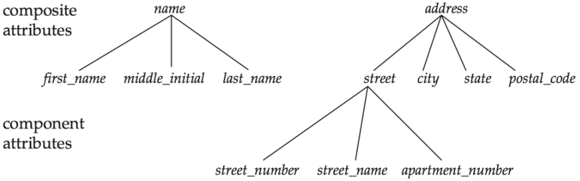
\includegraphics[height=0.8\textheight]{../Lecture 4.3_artifacts/image_000018_d53d875ecdc6b95c6474f4331f8126989ad6a0b0cc65de2fbae16071c4f89127.png}
    \end{center}
\end{frame}

\section{Entity Sets}
\begin{frame}
  \vfill
  \centering
  \begin{beamercolorbox}[sep=8pt,center,shadow=true,rounded=true]{title}
    \usebeamerfont{title}Entity Sets\par%
  \end{beamercolorbox}
  \vfill
\end{frame}

\begin{frame}{Entity Sets}
    \begin{itemize}
        \item An entity is an object that exists and is distinguishable from other objects.
        \begin{itemize}
            \item Example: specific person, company, event, plant
        \end{itemize}
        \item An entity set is a set of entities of the same type that share the same properties.
        \begin{itemize}
            \item Example: set of all persons, companies, trees, holidays
        \end{itemize}
        \item An entity is represented by a set of attributes; i.e., descriptive properties possessed by all members of an entity set.
        \begin{itemize}
            \item Example: \texttt{instructor = (ID, name, street, city, salary)}, \texttt{course = (course\_id, title, credits)}
            \item A subset of the attributes form a primary key of the entity set; that is, uniquely identifying each member of the set.
            \item Primary key of an entity set is represented by underlining it.
        \end{itemize}
    \end{itemize}
\end{frame}

\begin{frame}{Entity Sets instructor and student}
    \begin{center}
        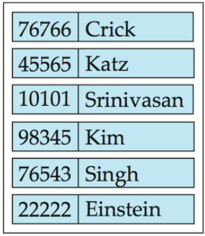
\includegraphics[width=0.45\textwidth]{../Lecture 4.3_artifacts/image_000021_1bc18f5766b782a3a9f47ae555ae9dbfb899323e56704197e19b201bff88e08f.png}
        \hfill
        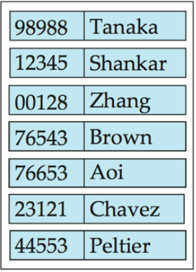
\includegraphics[width=0.45\textwidth]{../Lecture 4.3_artifacts/image_000022_219439696eef317f0329e46ed637754a084b8f1fd11c0897b29c4de227156bb1.png}
    \end{center}
\end{frame}

\section{Relationship}
\begin{frame}
  \vfill
  \centering
  \begin{beamercolorbox}[sep=8pt,center,shadow=true,rounded=true]{title}
    \usebeamerfont{title}Relationship\par%
  \end{beamercolorbox}
  \vfill
\end{frame}

\begin{frame}{Relationship Sets}
    \begin{itemize}
        \item A relationship is an association among several entities
        \item Example: \texttt{44553 (Peltier) -> advisor -> 22222 (Einstein)}
        \item A relationship set is a mathematical relation among $n \geq 2$ entities, each taken from entity sets
        \[ \{(e_1, e_2, \dots e_n) \mid e_1 \in E_1, e_2 \in E_2, \dots, e_n \in E_n\} \]
        where $(e_1, e_2, \dots e_n)$ is a relationship.
        \item Example: $(44553, 22222) \in \text{advisor}$
    \end{itemize}
\end{frame}

\begin{frame}{Relationship Set (2) advisor}
    \begin{center}
        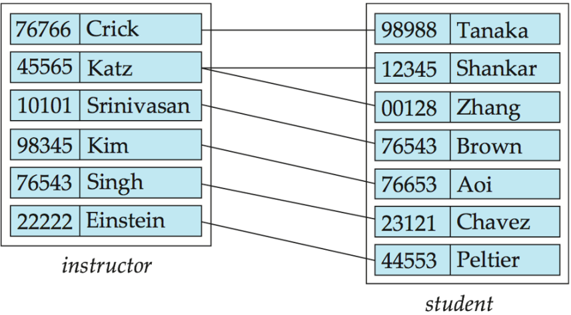
\includegraphics[height=0.8\textheight]{../Lecture 4.3_artifacts/image_000025_113e2a47865d68b951705055a41fdfc8aadc71c378ec4d5fd7f6521648cca349.png}
    \end{center}
\end{frame}

\begin{frame}{Relationship Sets (3)}
    \begin{itemize}
        \item An attribute can also be associated with a relationship set.
        \item For instance, the \texttt{advisor} relationship set between entity sets \texttt{instructor} and \texttt{student} may have the attribute \texttt{date} which tracks when the student started being associated with the advisor
    \end{itemize}
\end{frame}

\begin{frame}{Relationship Set (4): Degree}
    \begin{itemize}
        \item Binary relationship
        \begin{itemize}
            \item involves two entity sets (or degree two).
            \item most relationship sets in a database system are binary.
        \end{itemize}
        \item Relationships between more than two entity sets are rare. Most relationships are binary
        \begin{itemize}
            \item Example: students work on research projects under the guidance of an instructor.
            \item relationship \texttt{proj\_guide} is a ternary relationship between \texttt{instructor}, \texttt{student}, and \texttt{project}
        \end{itemize}
    \end{itemize}
\end{frame}

\begin{frame}{Attributes (3): Redundant}
    \begin{itemize}
        \item Suppose we have entity sets:
        \begin{itemize}
            \item \texttt{instructor}, with attributes: ID, name, dept\_name, salary
            \item \texttt{department}, with attributes: dept\_name, building, budget
        \end{itemize}
        \item We model the fact that each instructor has an associated department using a relationship set \texttt{inst\_dept}
        \item The attribute \texttt{dept\_name} appears in both entity sets. Since it is the primary key for the entity set \texttt{department}, it replicates information present in the relationship and is therefore redundant in the entity set \texttt{instructor} and needs to be removed
        \item BUT: When converting back to tables, in some cases the attribute gets reintroduced, as we will see later
    \end{itemize}
\end{frame}

\section{Cardinality}
\begin{frame}
  \vfill
  \centering
  \begin{beamercolorbox}[sep=8pt,center,shadow=true,rounded=true]{title}
    \usebeamerfont{title}Cardinality\par%
  \end{beamercolorbox}
  \vfill
\end{frame}

\begin{frame}{Mapping Cardinality Constraints}
    \begin{itemize}
        \item Express the number of entities to which another entity can be associated via a relationship set.
        \item Most useful in describing binary relationship sets.
        \item For a binary relationship set the mapping cardinality must be one of the following types:
        \begin{itemize}
            \item One to one
            \item One to many
            \item Many to one
            \item Many to many
        \end{itemize}
    \end{itemize}
\end{frame}

\begin{frame}{Mapping Cardinalities}
    Note: Some elements in A and B may not be mapped to any elements in the other set
    \begin{center}
        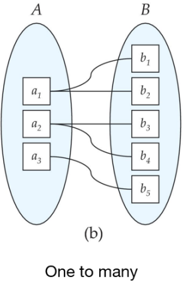
\includegraphics[width=0.45\textwidth]{../Lecture 4.3_artifacts/image_000035_c5f69c5edfdb2a7126234f301639f9a7a5543d57a341bc8d70983b05a6501bc9.png}
        \hfill
        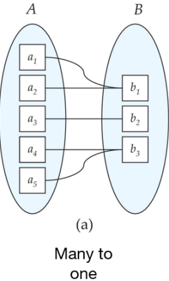
\includegraphics[width=0.45\textwidth]{../Lecture 4.3_artifacts/image_000037_158dcb3363c2014003faba30363115baf1342c7d2cebb1e6015bab23c00b60bd.png}
    \end{center}
\end{frame}

\begin{frame}{Mapping Cardinalities (2)}
    Note: Some elements in A and B may not be mapped to any elements in the other set
    \begin{center}
        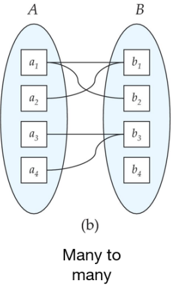
\includegraphics[width=0.45\textwidth]{../Lecture 4.3_artifacts/image_000038_447d7e7d664923f1a9c00bef0a981f6e37392e15e69521aaee7a2938215b6579.png}
    \end{center}
\end{frame}


\section{Weak Entity Sets}
\begin{frame}
  \vfill
  \centering
  \begin{beamercolorbox}[sep=8pt,center,shadow=true,rounded=true]{title}
    \usebeamerfont{title}Weak Entity Sets\par%
  \end{beamercolorbox}
  \vfill
\end{frame}

\begin{frame}{Weak Entity Sets}
    An entity set may be of two types:
    \begin{itemize}
        \item Strong entity set
        \begin{itemize}
            \item A strong entity set is an entity set that contains sufficient attributes to uniquely identify all its entities
            \item In other words, a primary key exists for a strong entity set
            \item Primary key of a strong entity set is represented by underlining it
        \end{itemize}
        \item Weak entity set
        \begin{itemize}
            \item A weak entity set is an entity set that does not contain sufficient attributes to uniquely identify its entities
            \item In other words, a primary key does not exist for a weak entity set
            \item However, it contains a partial key called as a discriminator
            \item Discriminator can identify a group of entities from the entity set
            \item Discriminator is represented by underlining with a dashed line
        \end{itemize}
    \end{itemize}
\end{frame}

\begin{frame}{Weak Entity Sets (2)}
    \begin{itemize}
        \item Since a weak entity set does not have primary key, it cannot independently exist in the ER Model
        \item It features in the model in relationship with a strong entity set. This is called the identifying relationship
        \item Primary Key of Weak Entity Set
        \begin{itemize}
            \item The combination of discriminator and primary key of the strong entity set makes it possible to uniquely identify all entities of the weak entity set
            \item Thus, this combination serves as a primary key for the weak entity set.
            \item Clearly, this primary key is not formed by the weak entity set completely.
            \item Primary Key of Weak Entity Set = Its own discriminator + Primary Key of Strong Entity Set
        \end{itemize}
        \item Weak entity set must have total participation in the identifying relationship. That is all its entities must feature in the relationship
    \end{itemize}
\end{frame}

\begin{frame}{Weak Entity Sets (3): Example}
    \begin{itemize}
        \item Strong Entity Set: Building (building no, building name, address). building no is its primary key
        \item Weak Entity Set: Apartment (door no, floor). door no is its discriminator as door no alone can not identify an apartment uniquely. There may be several other buildings having the same door number
        \item Relationship: BA between Building and Apartment
        \item By total participation in BA, each apartment must be present in at least one building
        \item In contrast, Building has partial participation in BA only as there might exist some buildings which has no apartment
        \item Primary Key: To uniquely identify any apartment
        \begin{itemize}
            \item First, building no is required to identify the particular building
            \item Second, door no of the apartment is required to uniquely identify the apartment
            \item Primary key of Apartment = Primary key of Building + Its own discriminator = building no + door no
        \end{itemize}
    \end{itemize}
\end{frame}

\begin{frame}{Weak Entity Sets (4): Example}
    \begin{itemize}
        \item Consider a \texttt{section} entity, which is uniquely identified by a \texttt{course\_id}, \texttt{semester}, \texttt{year}, and \texttt{sec\_id}.
        \item Clearly, \texttt{section} entities are related to \texttt{course} entities. Suppose we create a relationship set \texttt{sec\_course} between entity sets \texttt{section} and \texttt{course}.
        \item Note that the information in \texttt{sec\_course} is redundant, since \texttt{section} already has an attribute \texttt{course\_id}, which identifies the course with which the section is related.
    \end{itemize}
    \begin{center}
        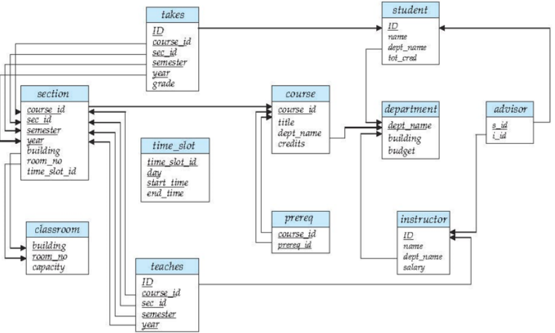
\includegraphics[width=0.6\textwidth]{../Lecture 4.3_artifacts/image_000044_0eb24be2f65adbd3f3744d6436b65322dd1493e1c0949ddd9a493a7b5b8bd411.png}
    \end{center}
\end{frame}

\begin{frame}{Module Summary}
    \begin{itemize}
        \item Introduced the Design Process for Database Systems
        \item Elucidated the E-R Model for real world representation with entities, entity sets, attributes, and relationships
    \end{itemize}
    \vspace{2em}
    \begin{center}
    \small \textit{Slides used in this presentation are borrowed from \url{http://db-book.com/} with kind permission of the authors.} \\
    \small \textit{Edited and new slides are marked with 'PPD'.}
    \end{center}
\end{frame}

\end{document}
